\section{Chebyshev不等式}
\label{sec:tail-chebyshev}

测量值会偏高也会偏低，我们常关心的是它离均值有多远，而不是越过哪一个固定阈值。偏离$X-\mu$可正可负，Markov不等式不能直接用；取绝对值或平方以后才非负。平方的好处是它的期望正是方差，一个最常知道的数。

\paragraph{转动惯量的论证}
继续把分布看成质量。方差$\operatorname{Var}(X)=\mathbb{E}[(X-\mu)^2]$是质量绕重心$\mu$的转动惯量：每块质量按到重心距离的平方加权。离重心至少$t$的质量，对转动惯量的贡献至少是“质量乘$t^2$”。转动惯量只有$\sigma^2$那么大，所以远离重心的质量至多是$\sigma^2/t^2$。

\begin{theorem}[Chebyshev不等式]
\label{thm:tail-chebyshev}
设$X$的方差有限，记$\mu=\mathbb{E}[X]$，$\sigma^2=\operatorname{Var}(X)$。则对每个$t>0$，
\begin{equation}
 \mathbb{P}(\lvert X-\mu\rvert\geq t)\leq\frac{\sigma^2}{t^2} .
 \label{eq:tail-chebyshev}
\end{equation}
\end{theorem}

这个结论称为\term{Chebyshev不等式}（Chebyshev inequality）。

\begin{proof}
因为$t>0$，两个非负数$\lvert X-\mu\rvert$与$t$的大小关系在平方后保持不变，所以两个事件相同：
\[
 \{\lvert X-\mu\rvert\geq t\}=\{(X-\mu)^2\geq t^2\} .
\]
$(X-\mu)^2$是非负随机变量，期望为$\sigma^2<\infty$。对它在阈值$t^2>0$处用定理~\ref{thm:tail-markov}，得到
\[
 \mathbb{P}\bigl((X-\mu)^2\geq t^2\bigr)\leq\frac{\mathbb{E}[(X-\mu)^2]}{t^2}=\frac{\sigma^2}{t^2} .
\]
两个事件相同，这就是式~\eqref{eq:tail-chebyshev}。
\end{proof}

压住示性函数的函数这次是抛物线，见图~\ref{fig:tail-dominating}(b)：$(x-\mu)^2/t^2$在$\lvert x-\mu\rvert\geq t$时不小于$1$，在其他地方不小于$0$。与直线相比，抛物线在两侧同时向上，所以一次控制住两个方向的偏离。

\paragraph{以标准差为单位}
当$\sigma>0$时，取$t=k\sigma$，式~\eqref{eq:tail-chebyshev}成为
\begin{equation}
 \mathbb{P}(\lvert X-\mu\rvert\geq k\sigma)\leq\frac{1}{k^2},\qquad k>0 .
 \label{eq:tail-chebyshev-k}
\end{equation}
它对每个方差有限的分布都成立。取$k=2$和$k=3$，任何这样的分布至少有$75\%$的质量落在均值两侧两个标准差以内，至少有$1-1/9\approx88.9\%$落在三个标准差以内。$k\leq1$时右边不小于$1$，不提供信息。

\paragraph{条件的作用}
定理只要求方差有限，不要求非负，也不要求对称。方差无穷时右边是$+\infty$，不等式没有内容；第~\ref{chap:common-distributions}章中自由度$\nu\leq2$的t分布就是这样，这时只能改用阶数更低的矩，见下一节。式~\eqref{eq:tail-chebyshev}控制的是双侧事件。单侧事件$\{X\geq\mu+t\}$包含在其中，所以同一个界也适用于单侧，只是不一定紧。

\paragraph{这个界同样不能再改进}
与Markov不等式一样，只知道均值和方差时，$\sigma^2/t^2$已经是最好的保证。设$0<\sigma\leq t$，构造三点分布：
\[
 \mathbb{P}(X=\mu-t)=\mathbb{P}(X=\mu+t)=\frac{\sigma^2}{2t^2},\qquad \mathbb{P}(X=\mu)=1-\frac{\sigma^2}{t^2} .
\]
它关于$\mu$对称，所以均值为$\mu$。偏离为$\pm t$的两点各贡献$t^2\cdot\sigma^2/(2t^2)$，合起来方差为
\[
 \operatorname{Var}(X)=2\cdot t^2\cdot\frac{\sigma^2}{2t^2}=\sigma^2 ,
\]
而$\mathbb{P}(\lvert X-\mu\rvert\geq t)=\sigma^2/t^2$，等号成立。

这个分布的形状与Markov的两点分布同出一辙：远处的质量恰好放在距离$t$处，一点也不再往外放，其余质量全部堆在中心，不贡献转动惯量。图~\ref{fig:tail-chebyshev-extremal}取$\mu=0$，$\sigma=1$，$t=2$，三点的质量为$1/8,3/4,1/8$，双侧尾概率是$1/4$；同样均值和方差的标准高斯分布，双侧尾概率只有$0.0455$。

\begin{BookInlineFigure}
 \centering
 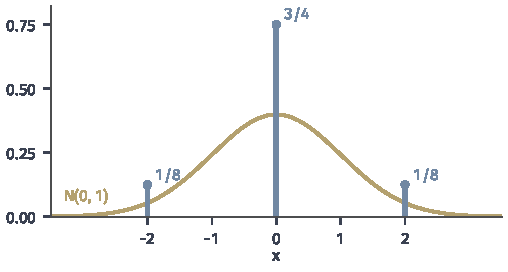
\includegraphics[width=86mm]{figures/07-probability/01-elementary-probability/matplotlib/tail-chebyshev-extremal/figure.pdf}
 \caption{使Chebyshev不等式取等号的三点分布（蓝色竖线，$\mu=0$，$\sigma=1$，$t=2$），质量$1/8,3/4,1/8$位于$-2,0,2$。黄线是均值、方差相同的$\mathcal{N}(0,1)$密度。}
 \label{fig:tail-chebyshev-extremal}
\end{BookInlineFigure}

\paragraph{与精确值比较}
由第~\ref{chap:common-distributions}章，贯穿例子的方差是$20\cdot\frac12\cdot\frac12=5$。取$t=5$，
\[
 \mathbb{P}(\lvert X-10\rvert\geq5)\leq\frac{5}{25}=0.2 .
\]
精确值是$0.0414$，界大了约五倍。单侧事件$\{X\geq15\}$也得到上界$0.2$，比Markov不等式的$2/3$好得多。改进来自两项新信息：方差告诉我们分布有多分散，均值作为中心使界只依赖偏离而不依赖原点的位置。

其他模型上可以看到同样的差距。对$Z\sim\mathcal{N}(0,1)$，
\[
 k=2:\ \tfrac14\ \text{对}\ 0.0455,\qquad k=3:\ \tfrac19\approx0.111\ \text{对}\ 0.0027 .
\]
对$X\sim\operatorname{Unif}(0,1)$，$\mu=1/2$，$\sigma^2=1/12$。$0<t\leq1/2$时精确值是$\mathbb{P}(\lvert X-1/2\rvert\geq t)=1-2t$。取$t=0.4$，精确值为$0.2$，界为$1/(12\times0.16)\approx0.521$。$t>1/2$时精确值是$0$，界却始终为正：Chebyshev不等式不知道分布的取值范围有界。

\paragraph{均值和方差不能决定尾部}
上面的比较说明，均值和方差相同的分布，尾部可以完全不同。图~\ref{fig:tail-same-variance}画出五个均值为$0$、方差为$1$的分布的双侧尾概率$\mathbb{P}(\lvert X\rvert\geq k)$：$[-\sqrt3,\sqrt3]$上的均匀分布，标准高斯分布，尺度为$1/\sqrt2$的Laplace分布，以及以各$1/2$概率取$\pm1$的两点分布。在$k=2$处，五个值分别是
\[
 0,\qquad 0.0455,\qquad \mathrm{e}^{-2\sqrt2}\approx0.0591,\qquad 0,\qquad \tfrac14 ,
\]
最后一个属于该处的三点极端分布。紫色曲线$1/k^2$是所有这些曲线的包络。

\begin{BookInlineFigure}
 \centering
 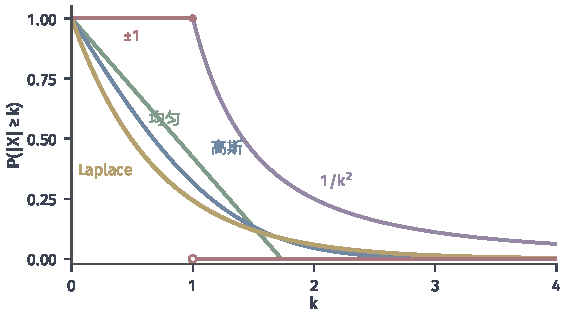
\includegraphics[width=96mm]{figures/07-probability/01-elementary-probability/matplotlib/tail-same-variance/figure.pdf}
 \caption{均值为$0$、方差为$1$的几个分布的双侧尾概率$\mathbb{P}(\lvert X\rvert\geq k)$。绿线为$[-\sqrt3,\sqrt3]$上的均匀分布，蓝线为$\mathcal{N}(0,1)$，黄线为尺度$1/\sqrt2$的Laplace分布，红线为取$\pm1$的两点分布，紫线为Chebyshev界$\min\{1,1/k^2\}$。}
 \label{fig:tail-same-variance}
\end{BookInlineFigure}

包络之下，曲线的形状由均值和方差之外的信息决定：均匀分布在$\sqrt3$处截断，两点分布在$1$处一下跳到零，Laplace分布的尾部比高斯分布更重。从$1/k^2$出发要把界进一步压低，就得知道分布在远处的更多情况，下一节用更高阶的矩来提供这样的信息。
